\chapter{ATLAS Detector: Further Details}
Further details here about the ATLAS detector are given.
\section{Muon subdetectors}
\subsection{RPC}
The RPCs offer fast triggering of the muons, providing track information in 15 to 25 ns. They are utilized in the barrel region ($|\eta|<1.05$) and made out of electrically resistive parallel plates with a 2mm distance filled with a gas mixture, arranged in three layers. The plates are kept at 9800 V potential difference to assure avalanche from the gas ionization caused by charged particles, which is then read out by metallic strips. The spatial resolution of this sub-detector is rather coarse, 10 mm in $\eta,\phi$ plane, which is the price to pay for the fast response.  

\subsection{TGC}
The TGC is again offering fast track information, but they are placed in the end-caps ($1.05<|\eta|<2.4$) and with four layers. The technology adopted here is the Multi Wire Proportional Chamber (MWPC). Typical readout happens in 25 ns.

\subsection{MDT}
The MDTs consist of pressurized drift tubes and, oppositely to the RPC and TGC, provides a high precision muon momentum measurement with a slower response. It is placed in $|\eta|<2.7$ and provides average spatial resolution of 80 $\mu$m, resulting in a total resolution of 35 $\mu$m, at the cost of charge collection time of 700 ns.
Tubes are arranged in three to eight layers within each chamber, enhancing the performance of tracking pattern recognition software.

\subsection{CSC}
The CSCs, like the TGC, are made out of MWPCs, covering the innermost end-cap ($2<|\eta|<2.7$), with resolution of 40 $\mu$m and a time resolution of 7 ns per plane, making them able to accommodate the higher particle flux due to the beam vicinity up to 1000 Hz/cm$^2$, making drift tubes technology infeasible to use in this region.

\section{L1}
The L1 exploits a raw information form the calorimeters and muons system, making use of algorithms to determine the Bunch Crossing Identification (BCID) associated to those raw measurements.
It then uses a custom-made electronics to take a decision in $\sim$ 25 $\mu$s on an event-by-event basis.
The raw information are simplified e.g. geometrically grouping together the calorimeter cells in so called \textit{towers}, while the muon system makes use of dedicated sub-detectors (RPC and TGC) as described above. The trigger information for the calorimeter (L1Calo) and the muon system (L1Muon) are then merged together. After that positive decision is made, the L1 defines one or more Region of Interest (RoI) which contains the measurements from the raw information and transmits those to the HLT.
\section{HLT}
At this step, in Run 1, the L2 trigger matched the inner detector data to the RoI, and made a successive trigger decision based on ID also, having $\sim$ 40 ms for this operation.
The selected events were then passed to the EF, which performed a full-granularity event reconstruction in the RoI, using hence all the sub-detector and not anymore raw data only, including calibrations, alignment corrections etc.
The EF had here 4 s for the final decision.
The computer resources were allocated separately to L2 and EF; in Run 2 instead this two step were reduced to 1 in the HLT, which is now a unique computer farm with merged processing nodes, for simplification and dynamic resources sharing.
If the event is again positive, it is registered on disk (here the final rate is 200 Hz) and will be then used for offline analyses. 
\section{Luminosity Measurement}
The delivered luminosity can be written as a function of the accelerator parameters as:
$$\mathcal{L}=\frac{n_Bf_rn_1n_2}{2\pi\Sigma_x\Sigma_y} $$
where $n_{1,2}$ are the numbers of protons per beam (1,2), $\Sigma_{x,y}$ characterize the horizontal and vertical convoluted beam width (measured through Van der Meer scans) and $f_r$ is the revolution frequency and $n_B$ is the number of bunches traveling at frequency $f_r$. There are also alternative parametrizations, where delivered luminosity is written as a function of the visible total inelastic cross section $\sigma_{vis}$ and the average number of inelastic interactions per bunch crossing $\mu_{vis}$.
A fundamental ingredient of the ATLAS strategy to assess  and  control  the  systematic  uncertainties  affecting  the
absolute luminosity determination is to  compare the measurements  of  several  luminosity  detectors,  most  of  which
use more than one algorithm to assess the luminosity. These
multiple detectors and algorithms are characterized by a significant different acceptance, response to pile-up, and sensitivity to instrumental effects and to beam-induced backgrounds.  


\chapter{Parton Shower and Hadronization Details}
\section{Parton Shower}
To perform a quantative study of the parton shower, one can start from the simple 2 $\to$ 2 process with the further splitting in into quarks and gluons, e.g. $q\to qg$, $g\to q\bar{q}$ and $g\to gg$. Parton shower can originate from initial state radiation (ISR) or final state radiation (FSR) like in Figure \ref{fig:factorization}. For details on this section, see \cite{partonshower}. 
The resulting process can now be depicted as $$2 \to 2 \otimes \textrm{ISR} \otimes \textrm{FSR}$$   
% It is important to note here that already the 2 $\to$ 2 process must be convoluted with the flux of incoming partons $i$ and $j$ in the two incoming protons, $A$ and $B$:
For the simplest 2 $\to$ 2 process, the production cross section is given by:
$$\sigma = \sum_{i,j}\iiint dx_1 dx_2 d\hat t f_i^A(x_1,Q^2)f_j^B(x_2,Q^2)\frac{d\hat{\sigma}_{i,j}}{d\hat{t}} $$
where $i$,$j$ are the incoming partons and $f_{i,j}^{A,B}(x_{1,2},Q^2)$ are the parton distribution functions of partons in the incoming protons, $A$ and $B$ and $Q^2$ being the momentum transfer squared.
The parton distribution function (PDFs) of gluons and sea quarks are strongly peaked at small momentum fractions $x_1 \sim E_i/E_A$, $x_2 \sim E_j/E_B$.  
The first step is to study the particular case of 2 $\to$ 3 e.g. with and additional gluon radiated from a quark in the final state.
Here the cross section can be written in the form \cite{halzenmartin}:
\begin{equation}
\frac{d\sigma_{2\to3}}{\sigma_{2\to2}}=\frac{\alpha_S}{2\pi}\frac{4}{3}\frac{x_1^2+x_2^2}{(1-x_1)(1-x_2)}dx_1dx_2
\end{equation}
\label{eq:sigma}
neglecting the quark masses. Now rewriting the energy fractions $x_j$ as $1-x_2=Q^2/E_{cm}^2$, $x_1\sim z$, $x_3 \sim 1-z$, equation \ref{eq:sigma} looks as follows:
$$d\mathcal{P}=\frac{d\sigma_{2\to3}}{\sigma_{2\to2}}\simeq \frac{\alpha_S}{2\pi} \frac{dQ^2}{Q^2}\frac{4}{3}\frac{1+z^2}{1-z}dz$$
\begin{wrapfigure}{r}{0.5\textwidth}
  \centering
      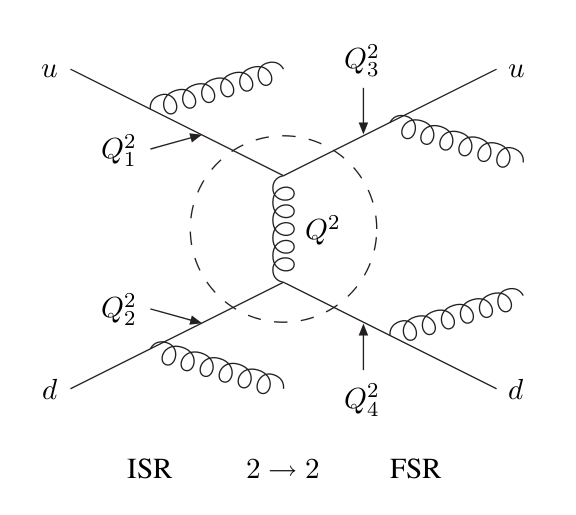
\includegraphics[width=0.45\textwidth]{/afsuser/fabnap/Documents/MasterArbeit/jet_part/factorization.png}
  \caption{Example of factorization of 2$\to n$ process.}
  \label{fig:factorization}
\end{wrapfigure}

which is collinear singular ($Q^2\sim 1-\textrm{cos}\theta\to 0$ if $\theta \to 0$ ).

To generalize the probability for the process $a\to bc$, which could be then gluon radiation ($q\to qg$) gluon splitting ($g\to gg$) or quark-antiquark splitting ($g\to q\bar{q}$), the Dokshitzer-Gribov-Lipatov-Altarelli-Parisi (DGLAP) equations are used:
$$d\mathcal{P}_{a\to bc}=\frac{\alpha_S}{2\pi} \frac{dQ^2}{Q^2}P_{a\to bc}(z)dz$$
where $P_{a\to bc}$ are fragmentation functions:
$$P_{q\to qg} = \frac{4}{3}\frac{1+z^2}{1-z} $$ 
$$P_{q\to gg} = 3 \frac{(1-z(1-z))^2}{z(1-z)} $$ 
$$P_{q\to q\bar{q}} = \frac{n_f}{2}(z^2+(1-z)^2) $$ 
and with $n_f$ being the number of quark flavors.

To describe now a cascade of successive branchings, like e.g. the one depicted in Figure \ref{fig:cascade}, one has to evolve the DGLAP equation above in smaller and smaller $Q^2$ using the so-called \textit{Sudakov factor} which describes  the probability that the \textit{first} emission happens at time $T$
$$d\mathcal{P}_{first}(T) = d\mathcal{P}_{sth}(T)\exp\left(-\int_0^T\frac{d\mathcal{P}_{sth}(t)}{dt}dt\right)$$
where $\mathcal{P}_{sth}$ is the probability of branching.

Thereby, the DGLAP equations become then
$$d\mathcal{P}_{a\to bc}(T) = \frac{\alpha_S}{2\pi} \frac{dQ^2}{Q^2}P_{a\to bc}(z) dz \exp\left(-\sum_b,c\int_{Q^2}^{Q^2_{max}}\frac{dQ^{'2}}{Q^{'2}}\int \frac{\alpha_S}{2\pi}P_{a\to bc}(z') dz'\right)$$
where the exponential term is called the Sudakov form factor and intuitively represents the probability of not having already radiated a particle with higher momentum transfer.
Sudakov formulation provides by definition the orderign in $Q^2$ (from larger to smaller) or in ``times'' from smaller to larger. By introducing the $Q^2_{max}$ as $Q^2$ of the hard-process one can regulate the collinear singularities.

% The advantage of the Sudakov formulation is that provides the ordering in $Q^2$ (from bigger to smaller values implies from smaller to bigger ``times'' i.e. later emission ) of the shower and that regulates the singularity for the first emission, if confronted with the procedure of using e.g. $\mathcal{P}_{q\to qg}$ multiple times. \\


\begin{wrapfigure}{l}{0.5\textwidth}
  \centering
      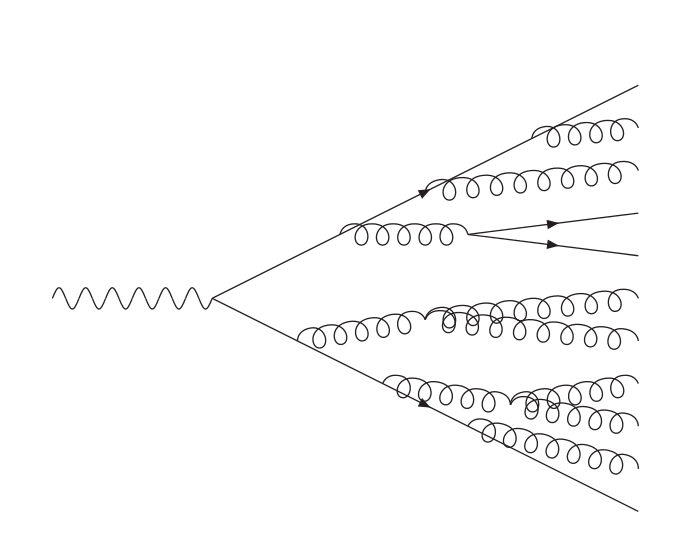
\includegraphics[width=0.35\textwidth]{/afsuser/fabnap/Documents/MasterArbeit/jet_part/cascade.png}
  \caption{Example of cascade of successive branchings.}
  \label{fig:cascade}
\end{wrapfigure}

Parton showers form ISR are described in similar way, but with the additional complication of taking into account the parton distribution functions.

Due to the asymptotic freedom, quarks and gluons resulting from the fragmentation described above, behave as quasi-free particles called partons, only at short distances (order of 10$^{-2}$ fm); when these colored objects separate more than the order of 1 fm, the confinement forces become effective, which have the effect of binding the quarks and gluons in hadrons. This process is referred to as \textit{hadronization}, which is a stochastic process involving a large number of particles, also described in the next section. The hadronization proceeds in fact through the formation of jet in high energy processes.

\section{Hadronization} % (fold)

Being non-perturbative, the process of hadronization is described with phenomenological models, the most important ones being: independent jet fragmentation, Lund string model and cluster hadronization.\\

In the first one, which is first one also historically in PETRA and PEP, gluonic flux tubes appear when colored objects separate and can then split to quark-antiquark pairs balancing they energy fraction and forming then primary mesons; the process lasts with the un-hadronized quarks and until the energy decreases to a cut-off. The problem of the model was an overall unsatisfactory implementation of the energy-momentum conservation, but had the advantage of a small number of parameters and simplicity.

In the (Lund) string model, which is similar to the independent fragmentation, $q\bar{q}$ interaction is described as string interaction with $V(r)\sim kr$, with $r$ being the distance, $k=|\frac{dE}{dz}|=|\frac{dp_z}{dz}|=|\frac{dE}{dt}|=|\frac{dp_z}{dt}|$ and neglecting the Coulomb part of the interaction. When tension reaches the critical values, the string breaks, forming new $q\bar{q}$ pair. See Figure \ref{fig:string} for a schematic representation. 

In the cluster model, hadronization mechanism is based on color pre-confinement; in fact gluons split to quark-antiquark pairs and nearby partons in cascade arrange themselves in color-neutral clusters, preferably at small invariant mass, down to the QCD scale, $\mathcal{O}$(200 MeV). With respect to the string model, it has the advantage of having a simple flavor composition with fewer parameters, but a less predictive energy-momentum description with more parameters.
\chapter{Topo-Clustering and Local Calibration Weighting}
\subsubsection{Topo-Clusters}
Topological cell clustering or topo-clustering, is the process where the calorimeter cells are grouped together in order to find energy deposited from the hard-scattering process. The result of topo-clustering is the formation of topo-cluster, in a way that suppresses calorimeter contribution from noise related effects, but still maintaining the activity from the underlying physical process.
The topo-clustering works as follow: first a seed cell is defined, and then other neighboring cells are added to the seed if their energy is above a noise threshold. 
% it starts with a seed cell and iteratively adds to the cluster the neighbor of a cell already in the cluster, provided that the energy in the new cell is above a threshold defined as a function of the expected noise. 
It is efficient at suppressing noise in clusters with large numbers of cells \cite{topocluster}. 

An additional step is taken to further reduce noise contribution, enhance the performance of topo-clusters and ensure that no bias is introduced in data: a local calibration scheme (Local Calibration Weighting, LCW) \cite{lcw} is also applied, based on Monte Carlo.

The calibration weights are determined from simulations of charged and neutral pions according to the cluster topology measured in the calorimeter. The cluster properties
used are the energy density in the cells forming them, the fraction of their energy deposited in the different calorimeter layers, the cluster isolation and its depth in the calorimeter.
\begin{wrapfigure}{R}{0.5\textwidth}
  \centering
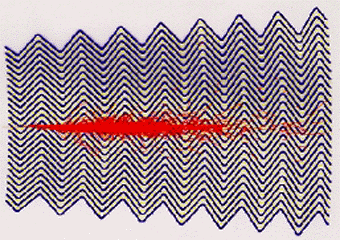
\includegraphics[width=0.45\textwidth]{/afsuser/fabnap/Documents/MasterArbeit/jet_part/images.png}
  \caption[Shower development in the accordion calorimeter]{Shower development in the accordion calorimeter, Monte Carlo simulation.}
  \label{fig:accordion}
\end{wrapfigure}
The natural requirement which has to be satisfied at this point is that the calorimeters cells should be then (three-dimensionally) ``grouped'' together, in order to reconstruct the energy of the hard-scattered particle. This is done in ATLAS in two steps: first the collection of calorimeter energy deposit represented as topo-clusters is created; then those objects are used as input for the jet reconstruction algorithm (here we are speaking of topo-clusters for the reconstruction of calorimeter jets; however other input can be tracks for track-jets and truth particles for truth-jets). 
Corrections are applied to the cluster energy to account for the energy deposited in the calorimeter, but outside of clusters and energy deposited in material before and in between the calorimeters. Jets are formed from calibrated clusters by using dedicated reclustering algorithms, described in the body of the thesis.

\chapter{Pile-Up and Underlying Event}
The \textit{pile-up} is a term used to describe the jets coming from another interaction in the same bunch-crossing (\textit{in-time pile-up}), i.e. coming form another interaction at low-$\pt$ which happens together with the hard-scattering, or in another bunch-crossing (\textit{out-of-time pile-up}), before or after the hard-scattering. When sub-detectors are sensitive to several bunch-crossing or their electronics integrate over more than 25 ns, these collisions can affect the signal in the collision of interest.

\begin{wrapfigure}{r}{0.5\textwidth}
  \centering
      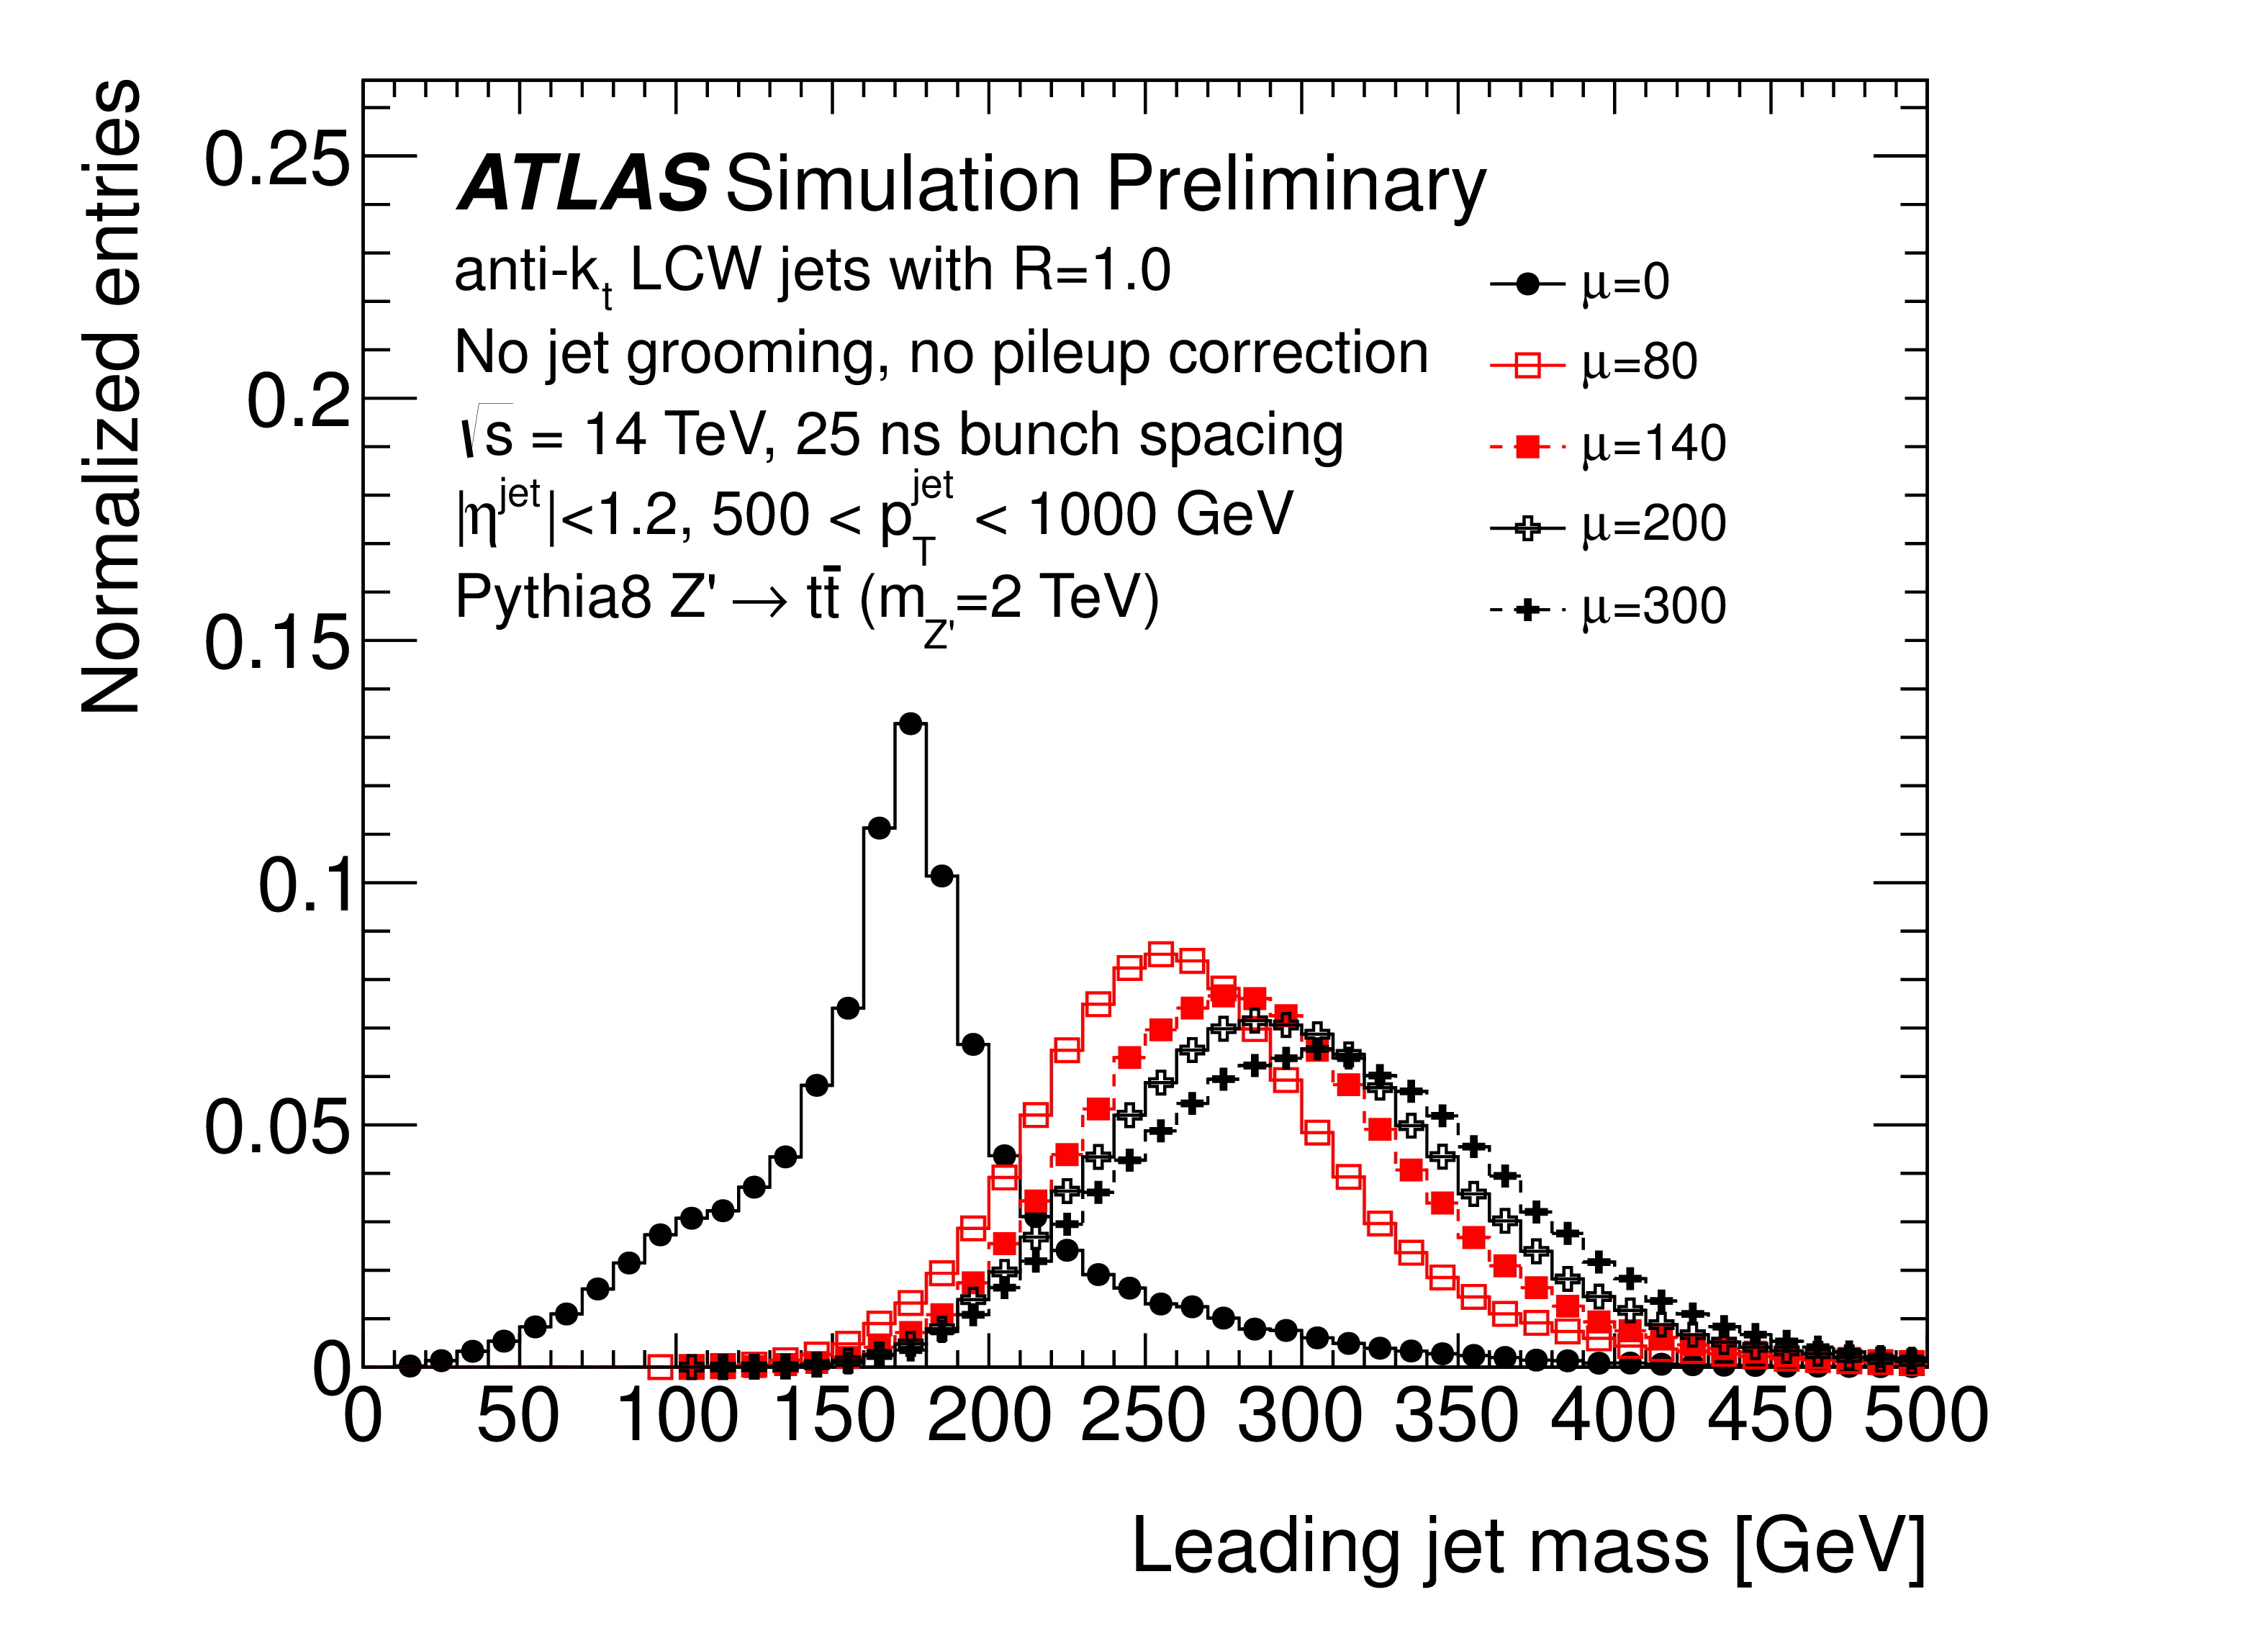
\includegraphics[width=0.5\textwidth]{/afsuser/fabnap/Documents/MasterArbeit/jet_part/Jet_ungroomed_mass_pt_500.png}
  \caption[Effect of pile-up contamination]{Effect of pile-up contamination in large-$R$ jets: here shown different PU conditions parametrized by $\langle\mu\rangle$. From \cite{highlumi}.}
  \label{fig:largejetpu}
\end{wrapfigure}


In case of the in-time pile-up, this effect can be directly parametrized by the number of primary vertices $N_{PV}$ reconstructed, which is around 15 for Run 2, and by the average number of interactions per bunch-crossing $\langle \mu \rangle$ (which is a function of the instantaneous luminosity $\mathcal{L}$) by the total inelastic cross section $\sigma_{in}$ and by the average frequency of bunch-crossing at the LHC $N_{bunch}\times f_{LHC}$:

$$\langle \mu \rangle = \frac{\mathcal{L}\times\sigma_{in}}{N_{bunch}\times f_{LHC}} $$

Given the increased luminosity condition for the Run 2, the average number of interactions is around 24, making the soft radiation contamination from PU an issue of increasing seriousness. 
The Underlying Event is a term which describes, in the single proton-proton interaction, all the phenomena, besides the hard-scattering, of several softer parton-parton scatters and the fragmentation of QCD strings which connects colored objects including beam remnant and initial and final state radiation \cite{ue}. Coming from the primary vertex, those soft radiations survive the tracks requirement to come from the PV (which is not the case for pile-up).

As seen in Figure \ref{fig:largejetpu}, where the large-$R$ jet mass is shown with five different PU conditions, the contamination spoils the distribution, giving rise to a misreconstruction which gets worse as it goes to worse environment conditions.\\

Other relatively small sources of contamination can be e.g. cavern background, beam halo events and beam gas events.


\begin{figure}
    \centering
    \begin{subfigure}[b]{0.45\textwidth}
	\centering
        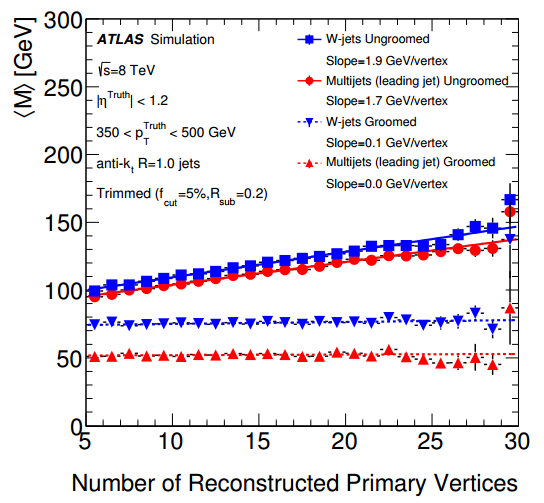
\includegraphics[width=0.78\textwidth]{/afsuser/fabnap/Documents/MasterArbeit/jet_part/grooming/pileup.png}
 
%         \label{fig:gull}
    \end{subfigure}
    \begin{subfigure}[b]{0.45\textwidth}
	\centering
        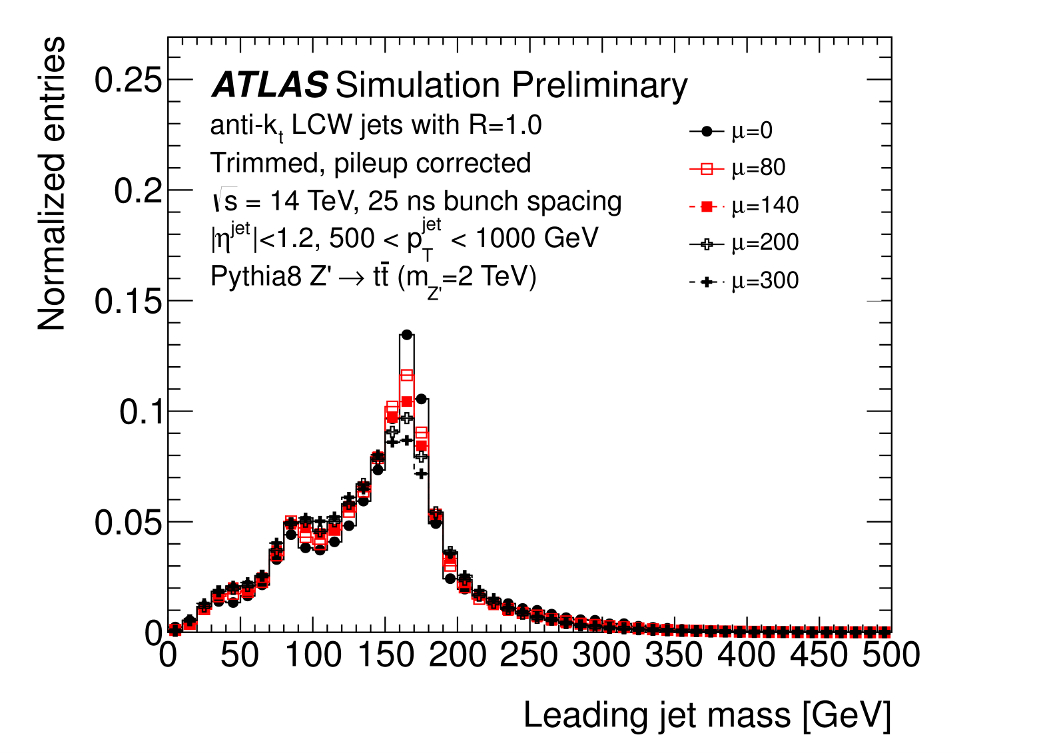
\includegraphics[width=\textwidth]{/afsuser/fabnap/Documents/MasterArbeit/jet_part/Jet_pileupcorrected_mass_pt_500.jpeg}
   
%         \label{fig:tiger}
    \end{subfigure}
    \caption[Effect of pile-up before and after trimming]{Left: mass reconstructed as a function of the number of primary vertices (parameterizing PU) for different samples; after trimming procedure the mass is pretty much independent of PU for all the samples. Right: mass distributions for different PU conditions: after trimming the reconstruction is not degraded as much as Figure \ref{fig:largejetpu}.} 
    \label{fig:trimmingperformance}
\end{figure}

\chapter{Additional Grooming Techniques}
The standard grooming technique used for the optimization studies of this thesis was described in the body; however there are two common choices which are worth mentioning here: the \textit{split-filtering} and the \textit{pruning}

\section{Split-Filtering}
The split-filtering was developed and optimized using C/A in jet searches of Higgs to \textit{b}-quarks. It is made out of two stages: the \textit{Mass-drop and symmetry} and the \textit{Filtering}.
For the Mass-drop and symmetry these are the steps:
\begin{itemize}
 \item the last step of C/A is undone, obtaining two sub-jets (e.g. the ones that should contain the bottom quark from Higgs decay);
 \item a significant difference between the parent jet mass and the sub-jets $j_i$ is required: $m^{j_i}/m^{jet}<\mu_{frac}$;
 \item the two $\pt$ of the sub-jets are required to be relatively similar (symmetry requirement) by the condition $\frac{min[(p_T^{j_1})^2,(p_T^{j_2})^2]}{(m^{jet})^2}\times \Delta R^2_{j_1,j_2} > y_{cut}$.
\end{itemize}
If the mass-drop and symmetry criteria are not satisfied, the jet is discarded.
The second step is the filtering:
\begin{itemize}
 \item $j_1$ and $j_2$ are reclustered with the C/A algorithm with variable radius parameter $R_{filt}=min[0.3,\Delta R^2_{j_1,j_2}/2]$, where $R_{filt}<\Delta R^2_{j_1,j_2}$;
 \item the jet is then filtered: all the constituents outside the three hardest sub-jets are discarded, in order to allow the emission of an additional radiation from the two-body decay;
 \item the split-filtered jet is composed of those three sub-jets only.
\end{itemize}
This method shows powerful sensitivity to highly collimated decays.

\section{Pruning}
The pruning algorithm is widely used in CMS; it works in a similar manner as the trimming, removing constituents (not sub-jets) with a relatively small $\pt$, but additionally applying a veto on wide angle radiation. The procedure runs as follows:
\begin{itemize}
 \item the C/A or k$_t$ reclustering algorithms is run on the constituents of the parent jet;
 \item at each reclustering step, transverse momentum \textit{or} an angular requirement has to be satisfied: being $j_1$ and $j_2$ the constituents, either $p_T^{j_1}/p_T^{j_1+j_2}>z_{cut}$ or $\Delta R^2_{j_1,j_2}< R_{cut}\times (2m^{jet}/p_T^{jet})$;
 \item $j_1$ and $j_2$ are merged only if one or both of those criteria are met, else $j_2$ is discarded and the algorithm continues.
\end{itemize}

\chapter{Limitation of the $\mtas$}

In this Appendix, additional results on the limitation of the $\mtas$ based on MC studies without detector interactions are presented. In particular, the truth study presented for boosted $W/Z$ decay in the thesis is here extended for boosted top quark decays.

As seen on Figure \ref{fig:breakdown3}, the breakdown of the $\mtas$ shows that, in particular for the high transverse momenta regimes, the tracks are subjected to fast degradation which makes their combination with the calorimeter mass not anymore an advantage. 

This is a limitation which was expected and understood from the detector performance point of view, and here shows the impossibility, with the variables which are presented here $\mta$ and $\mtas$ to reach a competitive standpoint with the $\mcal$ in the extreme kinematic regime for the top quark decay.

In black, in fact, the performance of the $\mtas$ variable using tracks with detector effect and sub-jets without those effects, shows this intrinsic limit which takes place already at 1.5 TeV.

\begin{figure}[!ht]
  \centering
      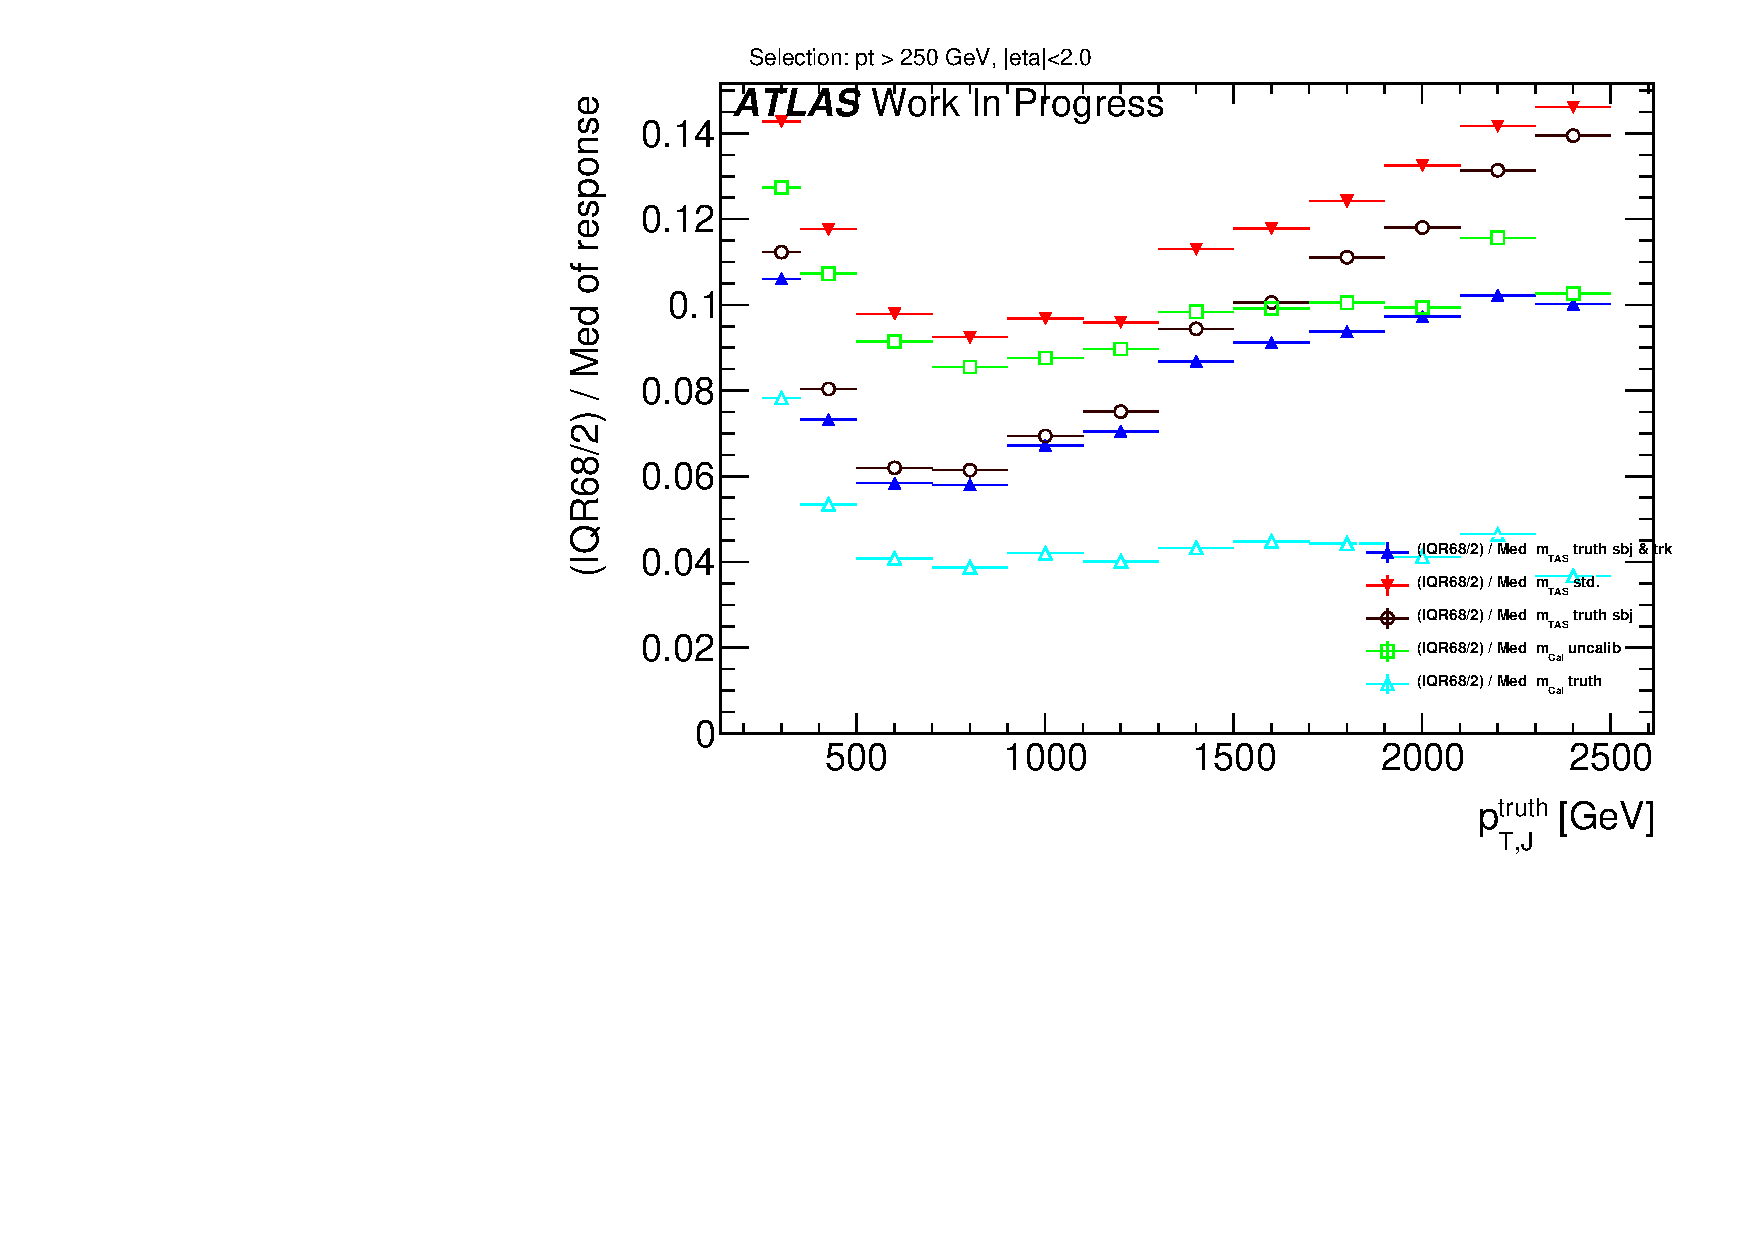
\includegraphics[width=0.7\textwidth]{/afsuser/fabnap/Documents/MasterArbeit/jet_part/appendixA/71graphcftr_h_JetRatio_mJ12CALOIQRoM4TruthsTops.pdf}
  \caption[Breakdown of the $\mtas$ ]{Breakdown of the $\mtas$ in its component using truth-level information for boosted top quarks decays.}
  \label{fig:breakdown3}
\end{figure}
